% introduction.tex
% Three-paragraph structure (language-audit pass, 2026-07-14; see
% project_language_audit_2026-07-14 memory):
% (1) synthetic data motivation, stylized facts, Fig 1;
% (2) survey of generative approaches and their failure modes on the
%     stylized facts, compacted into one comparison sentence;
% (3) single "In this study" contribution paragraph: hybrid HMM-WJ
%     (exhaustive metric/baseline list moved to Methods) folded
%     together with the multi-asset extension (variance correction +
%     diversification-return caveat, two sentences); VaR check moved
%     out (defined instead at its first true use in results.tex).

Synthetic financial data often fail to reproduce the statistical
properties of real returns. These paths are used to stress-test risk
models against unobserved market scenarios, validate portfolio
optimization algorithms, and Monte Carlo backtest allocators across
many independent scenarios~\cite{assefaEtAl2020, jordonEtAl2022}.
Empirical equity excess growth rates exhibit three statistical
regularities a generative model must reproduce: a heavy-tailed
marginal distribution, weak autocorrelation of raw growth rates, and
persistent volatility clustering, in which large changes are
followed by large changes and small changes by small changes~\cite{mandelbrot1963, cont2001, stengerEtAl2024}. All three patterns
are visible in SPY daily excess growth rates from $2014$--$2024$
(Fig.~\ref{fig:empirical_motivation}). These regularities, called
\emph{stylized facts}, are the benchmark for synthetic financial
data.

\begin{figure}[tbp]
    \centering
    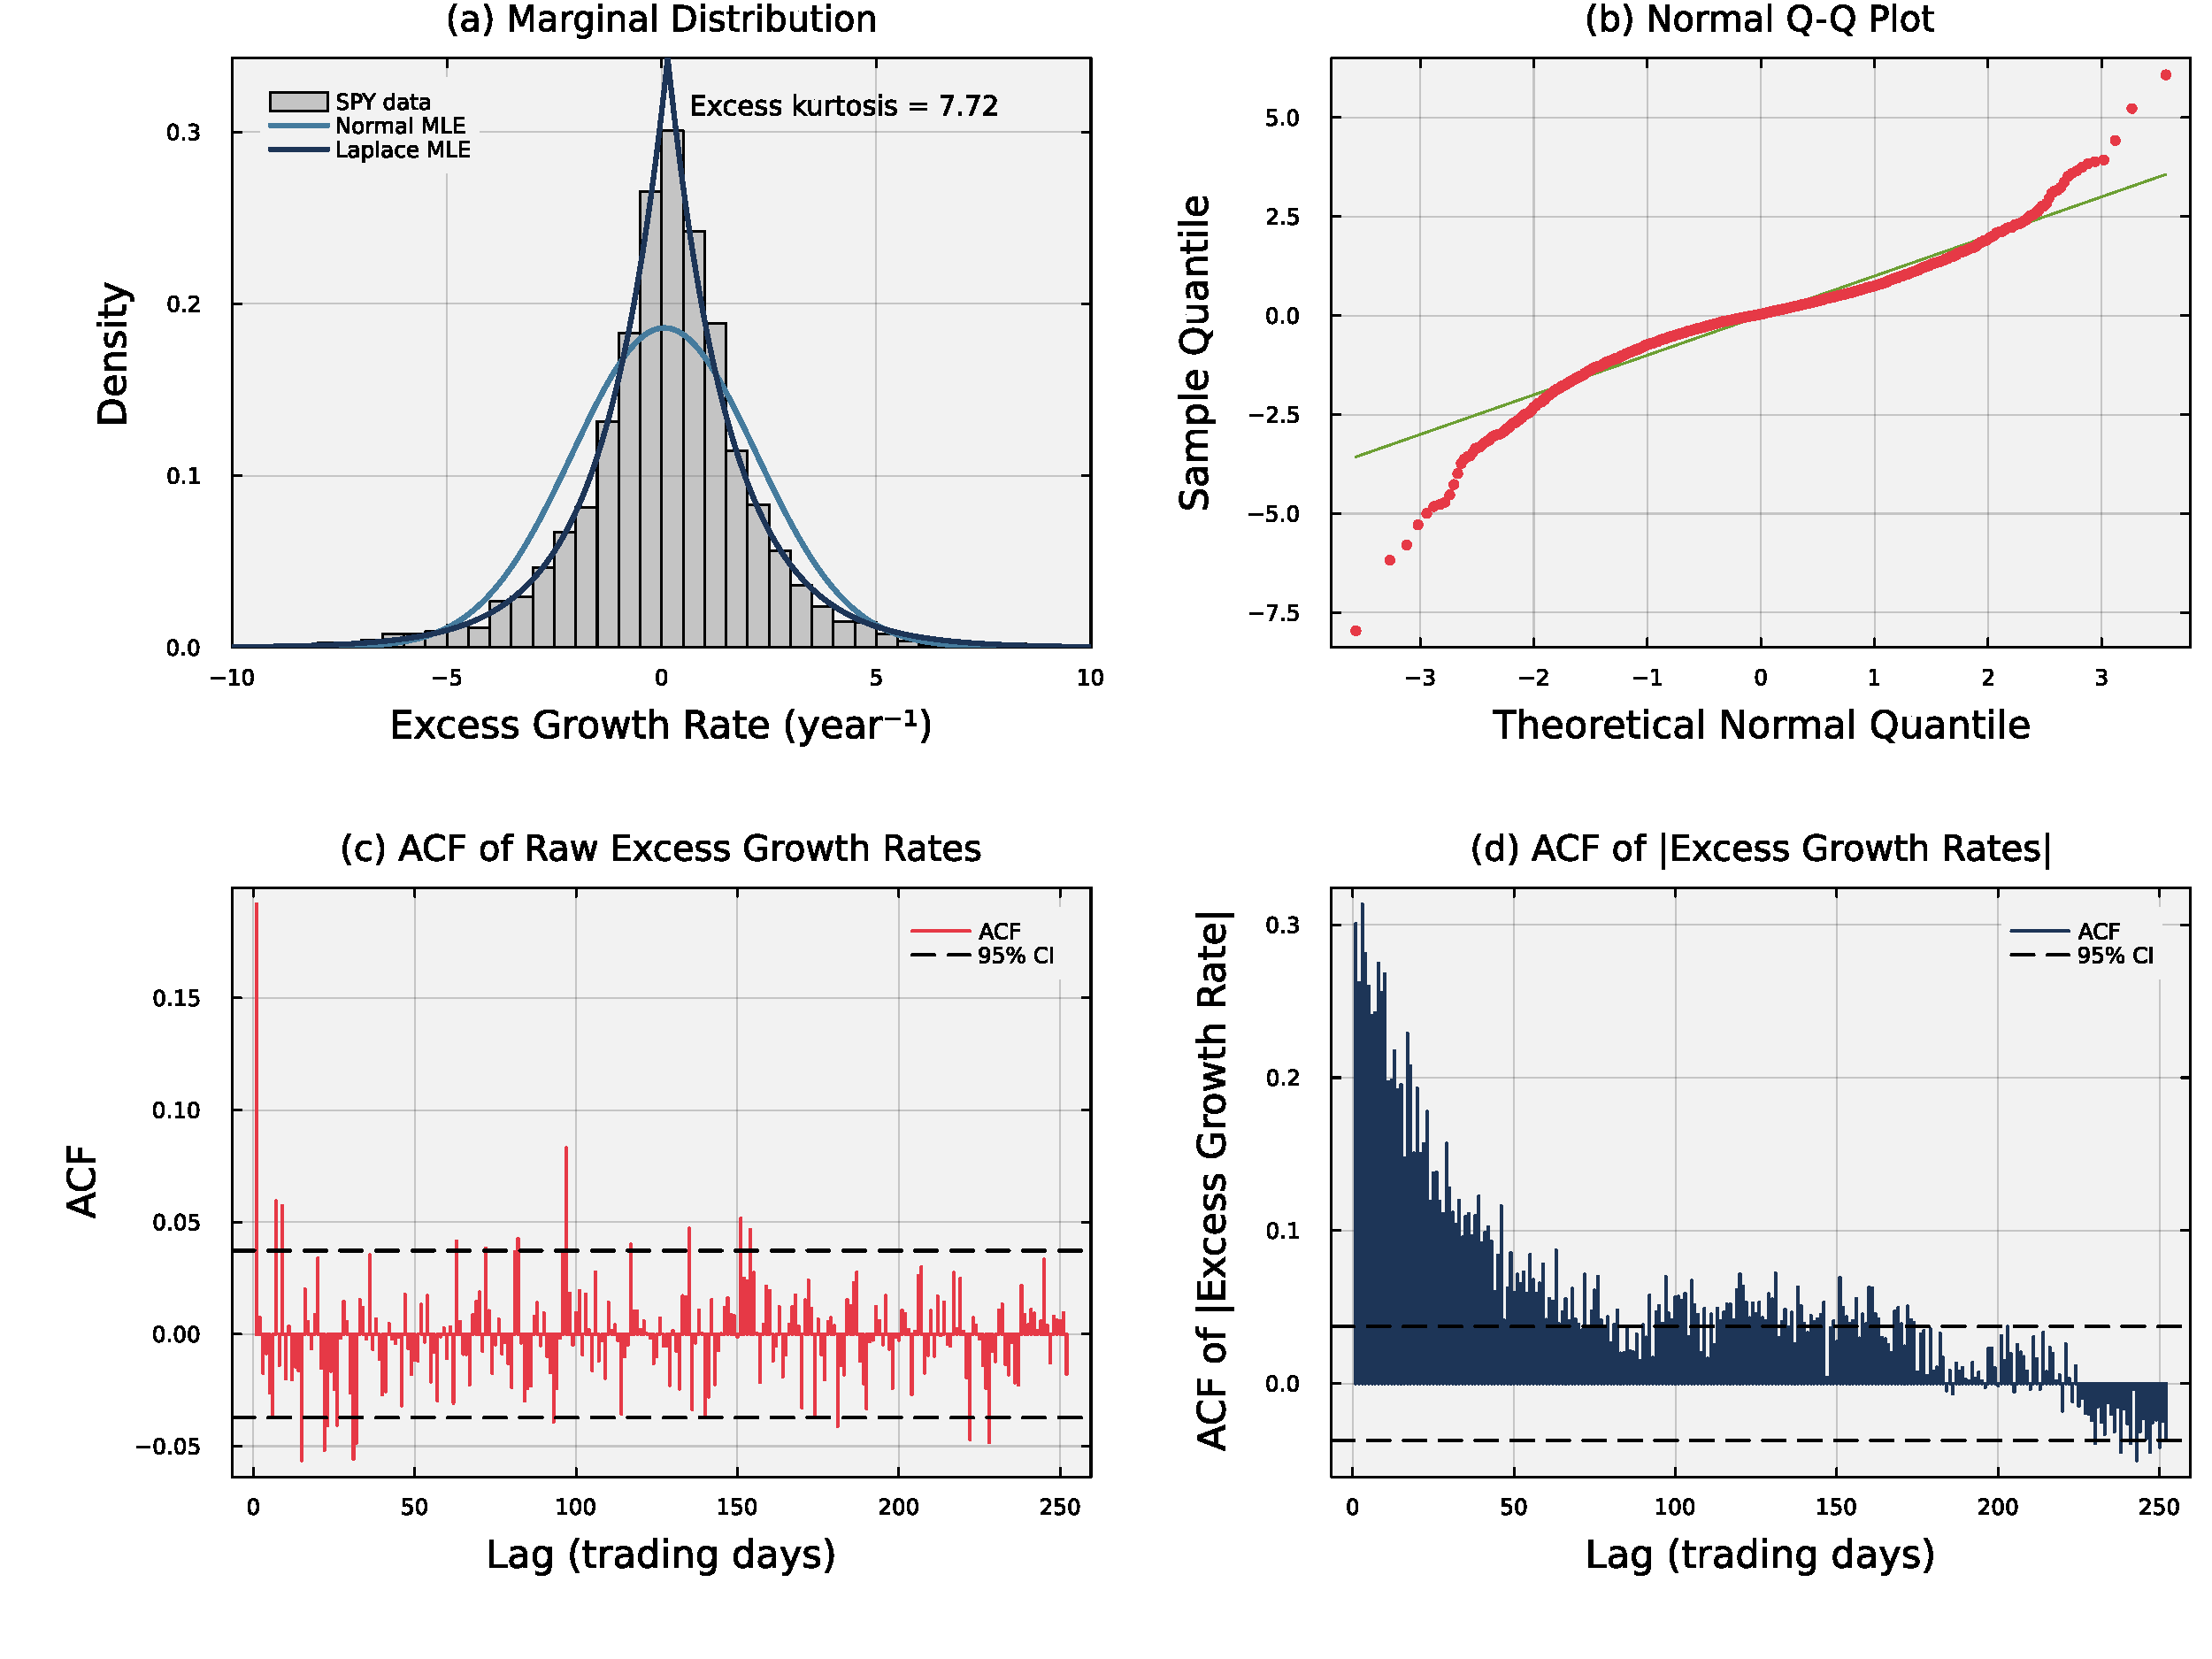
\includegraphics[width=\textwidth]{figs/Fig1-Empirical-Motivation.pdf}
    \caption{\textbf{Empirical stylized facts of SPY daily excess growth
    rates ($2014$--$2024$).} Panel~(a) shows the leptokurtic marginal
    density; the Laplace maximum-likelihood fit tracks the empirical
    peak and tails while the Gaussian fit does not. Panel~(b) confirms
    heavy tails through a normal quantile-quantile plot, with departure
    from the diagonal at both extremes. Panel~(c) shows the
    autocorrelation function of raw excess growth rates, which stays
    near zero across all lags and is consistent with the efficient
    markets hypothesis. Panel~(d) shows the autocorrelation function
    of absolute excess growth rates, which decays slowly and signals
    the persistent volatility clustering that the jump-duration
    extension is designed to reproduce.}
    \label{fig:empirical_motivation}
\end{figure}

Existing generative approaches typically reproduce some of these
regularities but not others. The generalized autoregressive
conditional heteroskedasticity (GARCH) family~\cite{engle1982,
bollerslev1986} captures volatility clustering but needs a
fat-tailed innovation to reproduce heavy tails; stochastic-volatility
and jump-diffusion models~\cite{heston1993, merton1976, kou2002}
enrich tail behavior but do not persist after a jump; deep generative
models~\cite{takahashiEtAl2019, yoonEtAl2019timegan, kwonLee2024}
learn complex marginals but routinely miss the absolute-return
autocorrelation that defines volatility clustering; and standard
hidden Markov models (HMMs)~\cite{rabinerJuang1986} offer a
regime-switching structure but revert to central regimes too quickly
to dwell in tail states long enough to reproduce the empirical
clustering profile~\cite{rydenTerasvirtaAsbrink1998, bullaBulla2006}.
We therefore sought a model that retained distributional fit while
improving volatility persistence and remaining practical for large
asset universes.

In this study, we developed a hybrid hidden Markov model with a
jump-duration mechanism (HMM-WJ) that pairs a Laplace-quantile state
partition with a Student-$t$ emission and a Poisson-distributed
jump-duration override. The Laplace partition lets the transition
matrix be estimated by direct frequentist counting rather than the
iterative Baum-Welch algorithm~\cite{baumPetrieSoulesWeiss1970,
bilmes1998}, which scales to a $424$-asset universe. We fitted the
model to a decade of SPY history, held out $2025$ for out-of-sample
evaluation, and scored the synthetic paths against seven baseline
generators on distributional and temporal fidelity. Relative to a
no-jump variant, HMM-WJ retained high distributional fit while
improving volatility-clustering fidelity, though GARCH remained the
strongest baseline on that dimension; HMM-WJ is therefore a tradeoff
between marginal and temporal fit rather than a uniformly better
model. Extending the
model to multi-asset applications required correcting
a known limitation of single-index composition, in which drawing
each asset's residual from a per-asset generator inflates the
composed marginal's variance quadratically in the factor loading; we
derived a closed-form scale correction that restores each ticker's
target variance after factor composition, recovering each ticker's
calibrated factor loading while retaining heavy-tailed returns.
Independent per-asset
residuals also exaggerate the daily cross-sectional spread among
assets, so daily-rebalanced portfolios built from these paths can
overstate diversification gains; we report this bias and a
location-shift adjustment set to a long-run prior, but the
adjustment does not restore the missing cross-asset dependence.
